% this file is called up by thesis.tex
% content in this file will be fed into the main document

\chapter{Background} \label{ch2} % top level followed by section, subsection
In this Chapter, we clarify the vital principles of the machine learning field. We begin by showing various machine learning problems and available algorithms that we can use in each issue. After that, we give information about different evaluation metrics for each challenge and describe different parameters concerning the experimental setup in this thesis. We continue with a brief description of classification algorithms that are utilized afterwards within the proposition. Finally, we end this Chapter with an overview of sequence encoding for classification problems. 

% change according to folder and file names
\ifpdf
    \graphicspath{{X/figures/PNG/}{X/figures/PDF/}{X/figures/}}
\else
    \graphicspath{{X/figures/EPS/}{X/figures/}}
\fi

% ----------------------- State of the art ------------------------


\section{Machine learning}
People acquire new knowledge from prior experiences, and tools catch instructions produced by people, however, what if people can teach the tools to learn from historical data and do what humans can do and act much faster that's called \textit{machine learning}$-$still, its a lot more than just learning; its also about understanding and reasoning. Machine learning is a group of techniques that learn from the past (historical) data on how to forecast or predict things related to the future. It tries to memorize or detect patterns from historical data that would help to predict trends in the near time.

Machine learning has a wide range of types and tasks, and we introduce the most important types of it in this thesis. For all types, we set up the following notation, (\romannumeral 1) \textit{Input:} $\textbf{x} = (x_1, x_2, \dots, x_d)$ where $\textbf{x}$ is a $d$-dimensional vector of independent variables or attributes, e.g. customer application; (\romannumeral 2) \textit{Output:} $y$ is the dependent (or target) variable e.g. good or bad customer; (\romannumeral 3) \textit{Target function:} $f: X \to Y$ e.g. ideal credit approval formula; (\romannumeral 4) \textit{Data:} $(x_1, y_1), (x_2, y_2), \dots, (x_N, y_N)$ e.g. historical records; (\romannumeral 5) \textit{Hypothesis} $g: X \to Y$.

ML can be classified into three main classes: (\romannumeral 1) \textit{Supervised learning:} $(x,y)$ in the form of \textit{(input, correct output)} where historical data as input, e.g. event logs are available with its correct label, e.g. outcome. This type of learning can be split into two main problems: Firstly, \textit{classification} where ML algorithms (e.g. \textit{Random Forest, XGBoost, CatBoost, $\dots$,} etc.) learn how to predict \textit{categorical} values such as good or bad; Secondly, \textit{regression} where ML techniques ( e.g. \textit{Linear regression, Ridge Regression,} $\dots$, etc.) predict a numerical and continuous value such as a price of the house; (\romannumeral 2) \textit{Unsupervised learning:} $(x, ?)$, in the form of \textit{(input, ?)} where historical data as input, e.g. users and movies characteristics are given with no information about the target label at all. In this type, we don’t predict a particular label regarding the input data. Still, we learn how to extract hidden structures from the give data (e.g. \textit{k-means}, i.e. Clustering algorithm), e.g. group customers to high/med/low level; (\romannumeral 3) \textit{Reinforcement learning} which is an intriguing type of learning because  it represents the human's  experience in learning, e.g. toddler learn to not touch a cup of tea that have smoke coming out of it. It's mostly used in games where an agent is in a place where it should take a set of \textit{actions}, and based on the action; the agent will be \textit{rewarded.} It takes the form of $(x, \hat{y} \subset  y,$ grade), i.e. \textit{(input, some output, a grade for this output).} Most machine learning methods assume that all attributes are \textit{numeric}. For \textit{categorical} ones we convert it to a numeric using different methods such as \textit{one-hot} encoding, however, in this thesis, we don’t need to do so since we introduce a machine learning method that can handle categorical features. 



\section{Machine learning work-flow.}
In this section, we introduce the general and basic work-flow for any ML project (see figure \ref{fig:ml1}), including the work on this thesis. (\romannumeral 1) At the beginning of an ML project, data preprocessing must be done, and mostly it takes most of the time, however in this thesis we used prepared data from \cite{teinemaa2019outcome} which represents $20$ real-life event logs from around $7$ different disciplines. (\romannumeral 2) Then we move forward with building a predictive model using different classification algorithms such as CatBoost. (\romannumeral 3) Splitting the historical data, e.g. event logs into \textit{training} (i.e. used to learn pattern form event log) and \textit{testing} (i.e. used to understand how the predictive model would perform in real-world cases) data sets. (\romannumeral 4) Tuning by splitting the training data further into a \textit{validation} (i.e. used to understand the predictive model behaviour on unseen data by calculating loss error then the model will adjust its parameter based on evaluation results on it) and training sets, this step is very important during the learning process, however in this thesis we used \textit{hyperopt} \cite{bergstra2013hyperopt} (i.e. a Python package to tune \textit{hyper-parameters} (i.e. variables we give to the algorithm during the learning process and can’t be learned, e.g. learning rate) of ML algorithm automatically) to do this step. (\romannumeral 5) The last and final step before deploying and delivering the predictive model to business organizations is the \textit{evaluation} of the resulted model after the training process.


\begin{figure}[htb]
	\begin{center}
		\resizebox{9cm}{!}{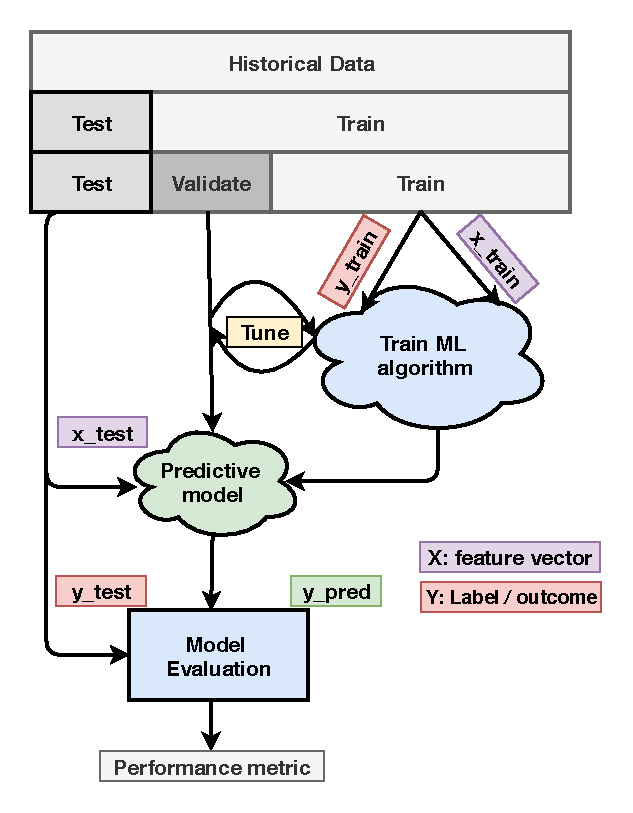
\includegraphics{images/general/ml1.pdf}}
		\caption[Machine learning workflow]{Machine learning workflow: split data into train, and validate sets to train and tune a machine learning model, in addition to a test set to evaluate this model}
		\label{fig:ml1}
	\end{center}
\end{figure}

\section{Evaluation metrics and experimental setups}
After building a predictive model, we evaluate it to decide if the resulting model is good enough to make predictions or not. To quantify the goodness or badness of classification models, we measure different evaluation metrics on test (or unseen ) data by comparing (see figure \ref{fig:ml1}) the predicted values (i.e. $y\_pred$) from the model with its true label (or baseline, i.e. $y\_test$). In the following subsection, we introduce different evaluation metrics. From now on, we discuss a binary classification problem i.e. $y \in \{1,0\}$ or $y \in \{+^{ve}, -^{ve}\}$.

\subsection{ Evaluation metrics} \label{auc}
A starting spot to quantify the goodness and badness of a classification model in ML could be a \textit{confusion matrix} (see figure \ref{fig:cm}). It shows the relation between correctly classified cases (or samples) and incorrectly classified cases. Confusion matrix split into four groups: (\romannumeral 1) \textit{True positives (TP)} which indicate to the actual true outcome (i.e. $y\_test$) was positive (i.e. $1$), and it’s predicted correctly (i.e. $y\_pred$, e.g. $1$) to be positive by the model; (\romannumeral 2) \textit{False positives (FP)} (i.e. \textit{type 1 Error}) refers to the actual true outcome was negative (e.g. $0$), and it’s assigned by the predictive model as positive; (\romannumeral 3) \textit{True negative (TN)} it means that actual true outcome was negative and the model predicts it correctly to be negative; (\romannumeral 4) \textit{False negative (FN)} (i.e. \textit{type 2 Error}) refers to the actual true outcome was positive, and it predicted incorrectly to be negative by the model. Using confusion matrix we get different \textit{metrics} to evaluate classification models such as \textit{accuracy}, i.e. relation between correctly classified cases and the total number of cases that are classified correctly and incorrectly, \textit{recall}, i.e. it gives information about how many models predict cases correctly out of all positive cases, \textit{precision}, i.e. how many cases that are positives, and model predict them successfully, and \textit{F-score} gives us the ability to measure precision and recall at the same time, and it uses \textit{harmonic mean} between them since it’s challenging to compare high recall with low precision together or vice versa.

\begin{figure}[htb]
	\begin{center}
		\resizebox{10cm}{!}{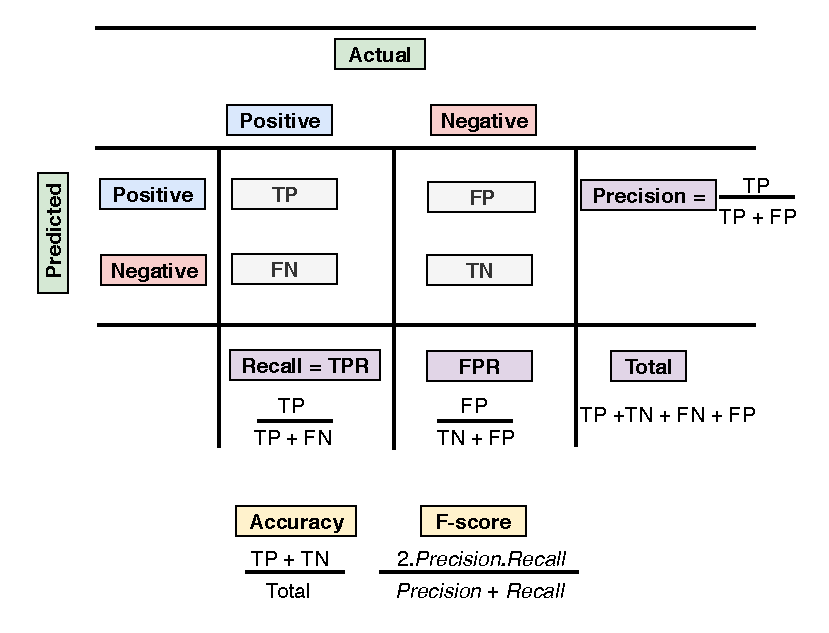
\includegraphics{images/general/cm.pdf}}
		\caption[Confusion matrix:]{Confusion matrix: represents the relation between actual outcomes and predicted cases. It contains different metrics that we use to evaluate any classification model, such as accuracy, F-score, etc.}
		\label{fig:cm}
	\end{center}
\end{figure}


The Most used metric in classification problems such as outcome-oriented PPM tasks is \textit{accuracy}. However, in many other cases, it’s not suitable to use it, such as when we have imbalanced outcomes where the majority of cases are negative in comparison to positive cases. In this situation, it’s recommended to use an \textit{F-score} that gives information about precision and recall at the same time.  All these metrics consider that the model will predict a binary number, i.e. one or zero based on the positivity or negativity of the predictions, however in many other cases the output from classifiers could be a probability estimation of the predicted outcomes and based on a threshold ($\alpha = 0.05$) we can assign each estimated value to a specific class, e.g. model predictions are $0.2$ and $0.8$ and based upon that we assigned $0.2$ to be negative and $0.8$ to be positive predictions.


Two more things that we can get from confusion matrix are (\romannumeral 5) \textit{True positive rate (TPR)} that is the same as recall and sometimes called \textit{sensitivity}; (\romannumeral 6) \textit{False positive rate (FPR)} that is opposite to recall, i.e. it gives information about how much a model predicts cases correctly out of all negative cases. We used in this thesis something else which is a widespread technique to evaluate classifiers that output a binary value score by building a  \textit{Receiver Operating Characteristics (ROC)} curve by plotting (see figure \ref{fig:roc}) pairs of TPR and FPR. Given a threshold  \textit{AUC}, i.e. the area under the ROC curve (or area under the curve) is mostly used to represent the relation between TPR and FPR as a single measured value. One of the most exciting benefits of using AUC as a single measure of outcome-oriented PPM over accuracy and F-score is that it keeps unbiased with imbalanced cases \cite{bradley1997use}. 

\begin{figure}[htb]
	\begin{center}
		\resizebox{10cm}{!}{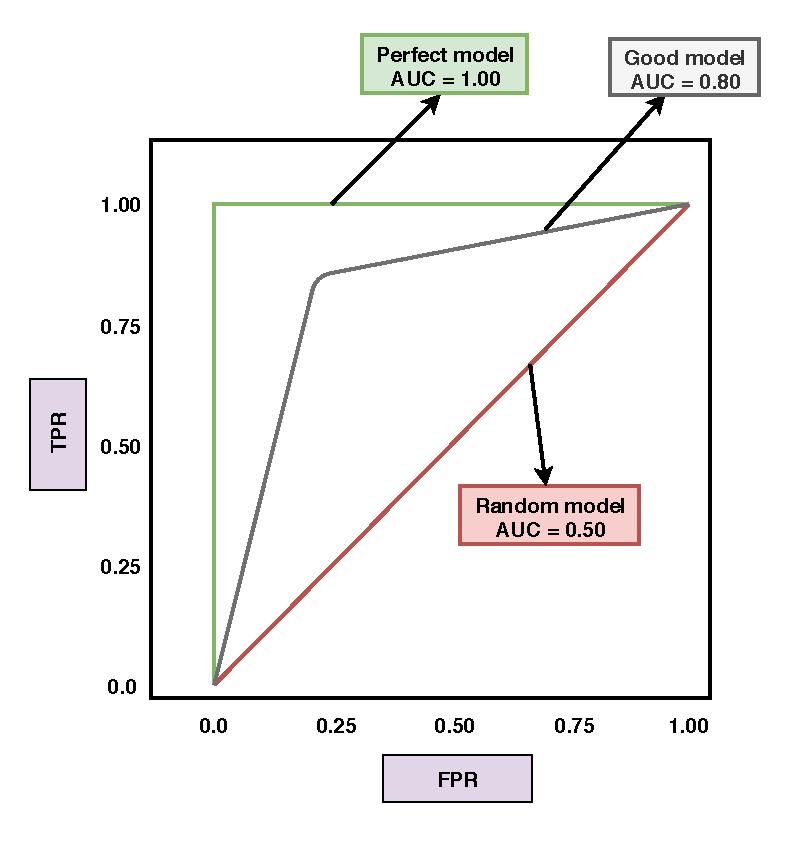
\includegraphics{images/general/roc.pdf}}
		\caption[ROC curve]{Receiver operating characteristics (ROC) curve show the relationship between the true positive rate (FPR) and the false-positive rate (FPR). The highest AUC the more robust predictive model.}
		\label{fig:roc}
	\end{center}
\end{figure}



\section{Classification algorithms}

In supervised ML, we have two main types of problems as mentioned earlier: classification and regression. In this thesis, we deal with outcome-oriented PPM, which is counted as a classification problem. In this part, we give an outline of different classification algorithms that are used in this thesis. We propose a recent classification algorithm to the area of outcome-oriented PPM, i.e. CatBoost with other four (e.g. XGBoost, Support Vector Machine, Random Forest, and Logistic Regression) classification algorithms from \cite{teinemaa2019outcome}.

\begin{enumerate}
	\item \textit{Decision trees:} DT is a type of supervised ml algorithms that is mostly used in classification tasks, but it can be used in regression tasks as well. DT is known as \textit{CART}, i.e. classification and regression tree.  A DT can be constructed as a flow chart since it has the same structure as it. The start and first node in a tree is the root node where each inner node indicates a test on each independent variable, and each division shows the outcome of that test, finally, the end node of the tree (or leaf node) carries a specific label, e.g. positive or negative. The advantages of CART are simple to understand, interpret, and visualize. DT performs a feature selection implicitly, and it can handle both numerical and categorical variables. The disadvantages of DT is \textit{over-fitting} (happens when the model learns data more than enough). DT can become uncertain because little changes of the data strength result in totally diverse produced trees, i.e. modification that requires to be lower by \textit{ensemble approaches (e.g. bagging and boosting)}. To construct a decision tree we want to decide about four main things: (\romannumeral 1) Which features to choose to start splitting; \textit{Information gain} is one of the methods that are used to choose between independent variables, and our target is to start splitting with features that have maximum information gain, i.e. capture more information. (\romannumeral 2) What condition for splitting; (\romannumeral 3) When to stop splitting; (\romannumeral 4) How to prune a tree to reduce the possibility of over-fitting; Trees are very useful when we use it with another superior machine learning methods such as Random Forest and Boosting (will be discussed later). DT has many parameters that we can tune such $max\_depth$ that defines the maximum size of a tree or how much deeper we can go in the tree which means with a large max depth we can do more splits and capture more information about the data. 
	
	\item \textit{Random Forest:} RF is a supervised ML algorithm worked with both classification and regression tasks and acts as a massive number of uncorrelated decision trees. RF uses \textit{bagging} (i.e. the mixture of learning models improves the classification efficiency) concept, and the principal purpose of bagging is to average boisterous and unbiased models to build a model including few variances. As the name implies, this method generates a forest with a number of decision trees, and in common the larger trees in the forest, the higher robust the prediction and moreover better accuracy. To model multiple decision trees to create the forest, we use the same methods of constructing the decision with the information gain as the DT algorithm.  In RF, we develop many trees as opposed to individual tree created in the CART method. To classify a distinct business process case based on all independent variables, every tree votes for a specific outcome class then the forest chooses the classification with the largest votes across all other trees in the forest. The advantages of RF classifiers are that they handle blowing values and preserve accuracy when a huge amount of the data are missing, handle large data sets with high dimensionality, and will not over-fit the model compared to DT. RF parameters that we can tune are the same as in decision trees, e.g. $max\_depth$, in addition to the \textit{number of iteration}, which represents the number of trees in the forest.
	
	
	
	
	\item \textit{Gradient Boosting:} GB is a type of machine learning algorithms that work well with heterogeneous data, i.e. does not have a specific internal structure and for this type of data gradient boosting is giving the best solution. In addition to the simplicity of using it. It is an iterative algorithm that is based on decision trees. GB is a group of ML procedures that contain multiple different algorithms such as \textit{XGBoost} (extreme gradient boosting), and \textit{CatBoost} (categorical boosting). It is estimated one of the common and most influential machine learning methods that can provide great results in terms of accuracy in many different practical tasks and can solve many complex data-driven real-life problems such as outcome-oriented PPM. These methods depend on the \textit{ensemble} (i.e. create many weak models to work together to create a very strong model) learning, and there are two main popular ensemble methods: (\romannumeral 1) \textit{Bagging} (see RF); (\romannumeral 2) \textit{Boosting}; In Boosting, predictive models are implemented in series, and in every progressive model the weights or the parameters are customized w.r.t the learning of the earlier model. GB is a special kind of boosting methods where it operates on decreasing faults sequentially and by tuning its parameters such as \textit{learning rate} (control the speed of learning process for each tree), $max\_depth$, \textit{number of iteration}, $\dots$, etc., we get very good results in terms of accuracy.  
	
	\item \textit{Logistic Regression:} LR is a  learning algorithm that we use when the outcome of the case is either positive or negative, i.e. binary value. This learning algorithm is considered as one of the simplest techniques for classification problems given set of independent variables $x= (x_1, \dots, x_m)$, the LR algorithm will calculate $\hat{y} = P(y=1 \mid x)$ by finding a linear combination of all independent variables (features) by giving each variable weight and sum the weighted sum of all features. $\forall x \sum_{i=1}^{m} w_i \cdot x_i + \epsilon $, where $w_i$ are model \textit{coefficients} and it's considered as a learnable parameter that LR algorithm can learn during the training process and $\epsilon$ is the \textit{intercept}. After that, the weighted sum is given to a sigmoid function $\sigma$ to convert it to an estimated probability value for both outcome classes such as $\sigma (\sum_{i=1}^{m} w_i \cdot x_i + \epsilon)$ . Fitted parameters such as coefficient, and intercept can be learned through optimizing a \textit{loss function}, e.g. \textit{cross-entropy loss} that measures how good our model is in only one training sample (or case), and to generalize this loss to all training cases we calculate \textit{cost function} which is the average losses of the entire training set. To learn these parameters automatically, we use a \textit{gradient descent optimization} algorithm to iterate over all coefficients (or weights) and update them during the training process. 

	\item \textit{Support Vector Machine:} SVM is a learning method which acts similarly to logistic regression when it comes to linear classification problems, in addition to the ability to do nonlinear classification through the \textit{kernel trick} that maps the data to a high dimensional feature vector. SVM works by discovering a \textit{hyperplane} that can separate the two classes. There are many hyperplanes that can be discovered using SVM, but the idea here is finding a plane with \textit{maximum margin}, i.e. maximum distance between cases for positive and negative class and \textit{hinge loss} is used to help with optimizing the maximum margin of SVM. In SVM we can optimize three different parameters to get better results in terms of accuracy: (\romannumeral 1) \textit{Kernel:} converting the input from a low dimensional space into a high dimensional space (e.g.  \textit{Radial Basis Function (RBF), sigmoid, polynomial, etc.)}; (\romannumeral 2) \textit{Regularization (C):} this parameter used to represent the error or misclassified cases, and it’s used with the decision boundary to control the trade-off between them; (\romannumeral 3) \textit{Gamma:} this parameter can be set with RBF kernel, and it refers to how far/close influence a single training case has \cite{platt1999probabilistic}.

\end{enumerate}

\section{Early classification and sequence encoding approaches}
About the extensive writing on ML, we found that the outcome-oriented PPM belongs to the task of an early sequence classification problem. It means, given a collection of sequences with its outcome (or label), the target is to define a function $F$ that for each sequence prefix it predicts the outcome of w.r.t this prefix. 

In recent years, early sequence classification approaches are by and large centred on identifying a \textit{prefix length} that gives a reasonable prediction \cite{xing2012early}.  In literature, methods to define the range of prefixes are many and different. For example \cite{mori2017reliable}, they built a way that helps with early sequence prediction problems that depend on the relation between accuracy of the prediction for the prefix and accuracy for the full sequence.  

Outcome-oriented PPM is considered as a problem of an early sequence classification with \textit{complex sequence encoding} (i.e. a stream of events with payload attributes) of the event logs \cite{santos2016literature, xing2010brief}.  Complex sequence encoding methods are proposed in \cite{leontjeva2016complex} where it used in place of \textit{simple sequence encoding} (i.e. a stream of events without payload) to deal with outcome-oriented prediction problems, the complexity space of the prediction problem increases significantly \cite{di2017eye}. A few works have been done on early sequence classification over complex sequence encoding, for example \cite{lin2015reliable}, where they develop a serial decision tree to determine the length of prefixes. A few of the baselines of dealing with complex sequence encoding utilize \textit{index-based} encodings \cite{leontjeva2016complex}.  Complex sequence encoding permits us to encode an event log, to capture as much data as conceivable whereas having a structure that effectively can be utilized with standard machine learning algorithms.

%add figures
%\begin{figure}
%\centering
%\includegraphics[width=0.65\textwidth]{2/figures/Cloud/funambolArchitecture.png}
%\caption{Funambol architecture}
%\label{fig:funambolArchitecture}
%\end{figure}


% ---------------------------------------------------------------------------
% ----------------------- end of thesis sub-document ------------------------
% --------------------------------------------------------------------------- 